%% Ez a fájl felelős azért, hogy beállítsa, hogy hogyan nézzen ki a dokumentum, leírja az összes formázást. A fájl végén található rész pedig elindítja a pdf generálását a contents.tex importálásával.

% Általános formázások
% -------------------------------------------------------

% twoside: kétoldalas nyomtatás --> írd át oneside-ra, ha egyoldalasan nyomtatod (de ne nyomtasd egyoldalasan, mert a TVSZ is kétoldalas nyomtatást javasol)
% 11pt: betűméret
\documentclass[a4paper,11pt,twoside]{report}

% Betűtípus váltása
%\renewcommand{\familydefault}{ppl}
% További betűtípusok: https://www.sharelatex.com/learn/Font_typefaces

% Tartalomjegyzék formázásához
\usepackage{tocloft}
% Tartalomjegyzékben az al-alfejezetek (\section) indentálása
\setlength{\cftsecindent}{.9cm}
% Tartalomjegyzékben az al-alfejezetek (\subsection) indentálása
\setlength{\cftsubsecindent}{1.4cm}

% Ezzel ha két bekezdés közé üres sort teszel, akkor a kimeneti pdf-ben is megjelenik térköz a két bekezdés közt
%\usepackage{parskip}
% -------------------------------------------------------


% Fejezetcímek formázása
% -------------------------------------------------------
\usepackage{titlesec}

% Milyen mélységig legyenek számozva az fejezetek
% 0: csak a fejezetek (\chapter) vannak számozva (bevezetés, irodalomkutatás stb.)
% 1: alfejezetek (\section) is számozva vannak
% 2: al-alfejezetek (\subsection) is számozva vannak
\setcounter{secnumdepth}{2} 

% Fejezetcímek formázása
\newcommand{\titleformatting}{
    % Közvetlenül a fejezetcím előtt legyen a szám, "fejezet" szó pedig nem kell.
    %\titleformat{\chapter}{\normalfont\huge}{\thechapter.}{1em}{\huge\textbf}
    
    % Maradjon a két soros fejezetcím (1. fejezet, és új sorban a fejezetcím), viszont a -5pt lecserélésével állítható az "1. fejezet" és a fejezetcím közti térköz
    %\titleformat{\chapter}[display]{\normalfont\huge\bfseries}{\thechapter.\ \chaptertitlename}{-5pt}{\Huge}
    
    % Fejezetcím körüli térköz módosítása (a 0pt a bal oldali térköz, a -10pt a fejezetcím előtti, az 5pt pedig az utáni térköz
    % FONTOS! Ez a beállítás csak akkor működik, ha a fenti titleformat parancsok közül valamelyik elől kitörlöd a kommentjelet.
    %\titlespacing{\chapter}{0pt}{-10pt}{5pt}
}
%\titleformat{\chapter}[display]   
%{\normalfont\huge\bfseries}{\chaptertitlename\ \thechapter}{20pt}{\Huge}

% Az alfejezet-címek (\section) száma előtt ne szerepeljen a fejezet (\chapter) száma (pl 2.1 helyett csak simán 1)
%\renewcommand\thesection{\arabic{section}}

% Alfejezetcímek formázása:
%\titleformat{melyik elem}[block/wrap]{számozás formázásai}{számozás maga}{térköz a számozás és a cím között}{cím formázásai}
% méretek: \large, \Large, \huge, \Huge
% további formázási lehetőségek: \bfseries (vastag), \it (dőlt), \underline (aláhúzott)
% \thesection: Az adott cím sorszámát helyettesíti be (épp ezért kell a pont a \thesection parancs után, hogy a cím sorszáma után legyen pont)
\titleformat{\section}[block] {\normalfont\Large\bfseries}{\thesection.}{1em}{\Large}
% -------------------------------------------------------


% Kötelező formázás
% -------------------------------------------------------

% margók
\usepackage[margin=2.5cm, bindingoffset=1.25cm]{geometry}

% másfeles sorköz
\linespread{1.5}
% -------------------------------------------------------


% Hasznos csomagok
% -------------------------------------------------------

% ékezetes betűk kezelése
\usepackage[utf8]{inputenc}

% ékezetes betűknél is legyen automatikus elválasztás
\usepackage[T1]{fontenc}

% nyelvi csomag
\usepackage[english, magyar]{babel}

% képletekhez kell
\usepackage{mathtools}                        

% bibliográfia (IEEE formátumban)
\usepackage[style=ieee, backend=biber]{biblatex}

% ez az ITK logó pozicionálásához kell
\usepackage[export]{adjustbox}

% kattintható tartalomjegyzék és hivatkozások
\usepackage[hidelinks, unicode, pdfusetitle]{hyperref}

% PDF könyvjelzők
\usepackage{bookmark}

% Színes cellák táblázatokban
\usepackage[table,xcdraw]{xcolor}

% Hyperlinks - URL-ek a szövegben
\usepackage{url}

% Hosszabb idézetek
\usepackage{csquotes}

% a bibliográfiában megfelelően legyenek formázva az idézőjelek
\DeclareQuoteAlias{german}{magyar}

% Kódrészletek
\usepackage{listings}
\usepackage{sourcecodepro} % egy jó betűtípus
\lstset{captionpos=b, numberbychapter=false, basicstyle=\ttfamily, showstringspaces=false, columns=fullflexible}

% Kódrészletek magyar stílusú számozása
\renewcommand\lstlistingname{kódrészlet}
\makeatletter
\renewcommand\fnum@lstlisting{\ifx\lst@@caption\@empty\else\thelstlisting.~\fi\lstlistingname}%
\makeatother

% Képek beszúrásakor automatikusan ebben a mappában fogja a képeket keresni
\graphicspath{ {images/} }

% Hivatkozásokat tartalmazó fájl
\addbibresource{hivatkozasok.bib}

% Random szövegek generálása - nyugodtan töröld
\usepackage{lipsum}

% Csak hogy ne sírjon amiatt, hogy a BibLatex 3.12-es verziója rengeteg változtatást tartalmaz az előző verzióhoz képest
\BiblatexHungarianWarningOff
% Ez meg egy másik felesleges warning-ot némít el (https://tex.stackexchange.com/a/451193)
\usepackage{silence}
\WarningFilter{biblatex}{File 'english-ieee.lbx'}
% -------------------------------------------------------

% Pdf fájlok beszúrásához, mint pl. a témabejelentő
\usepackage{pdfpages}


% Címoldal + üres lap utána
% -------------------------------------------------------
\author{\nev\\\kepzes}
\title{\Huge{\tipus}\\[1cm]
    \huge{\cim}}
\date{\the\year}

\newcommand{\cimlap}{
    
\includegraphics[valign=m, width=50pt]{ITK_logo} \parbox[c]{0.8\textwidth}{
    Pázmány Péter Katolikus Egyetem\\
    Információs Technológiai és Bionikai Kar}
    \vspace*{\fill}
    
    {\let\newpage\relax\maketitle}
    \vspace*{\fill}
    \begin{center}
    \bigskip
    
    \temavezetok
    \end{center}
}

\newcommand{\ureslap}{
    \begingroup
        \pagestyle{empty}
        \cleardoublepage
    \endgroup
    \clearpage
}
% -------------------------------------------------------


% ------------- Dokumentum legenerálása -----------------
\begin{document}

\titleformatting

% Ez a fájl felelős azért, hogy a projekt fájljait összefűzze egy kimeneti pdf-fé.

% Ezeket írd át...
\def\tipus{SZAKDOLGOZAT} % --> ha MSc-s vagy, írd át "DIPLOMAMUNKA"-ra!
\def\nev{Juhász Bence}
\def\kepzes{mérnökinformatikus BSc}
\def\cim{Multimodális, AI-alapú ételfelismerés pontosságának optimalizálása}
\def\temavezetok{Témavezető: Dr.\ Tornai Kálmán}

% címlap generálása
\cimlap

% A kötelező részeket római oldalszámozással tünteti fel a tartalomjegyzékben. Ha nagy betűvel írod a "Roman"-t, akkor nagy római számokkal fog számozni.
\pagenumbering{roman}

% Kötelező részek
% Ha nem szeretnéd ezeket a részeket feltüntetni a tartalomjegyzékben, akkor egyszerűen töröld az \addcontentsline kezdetű sorokat.
\addcontentsline{toc}{chapter}{Témabejelentő}

% Hogy kétoldalas nyomtatás esetén a témabejelentő közvetlenül a címlap után lehessen
% \ureslap

% A témabejelentő beszúrása
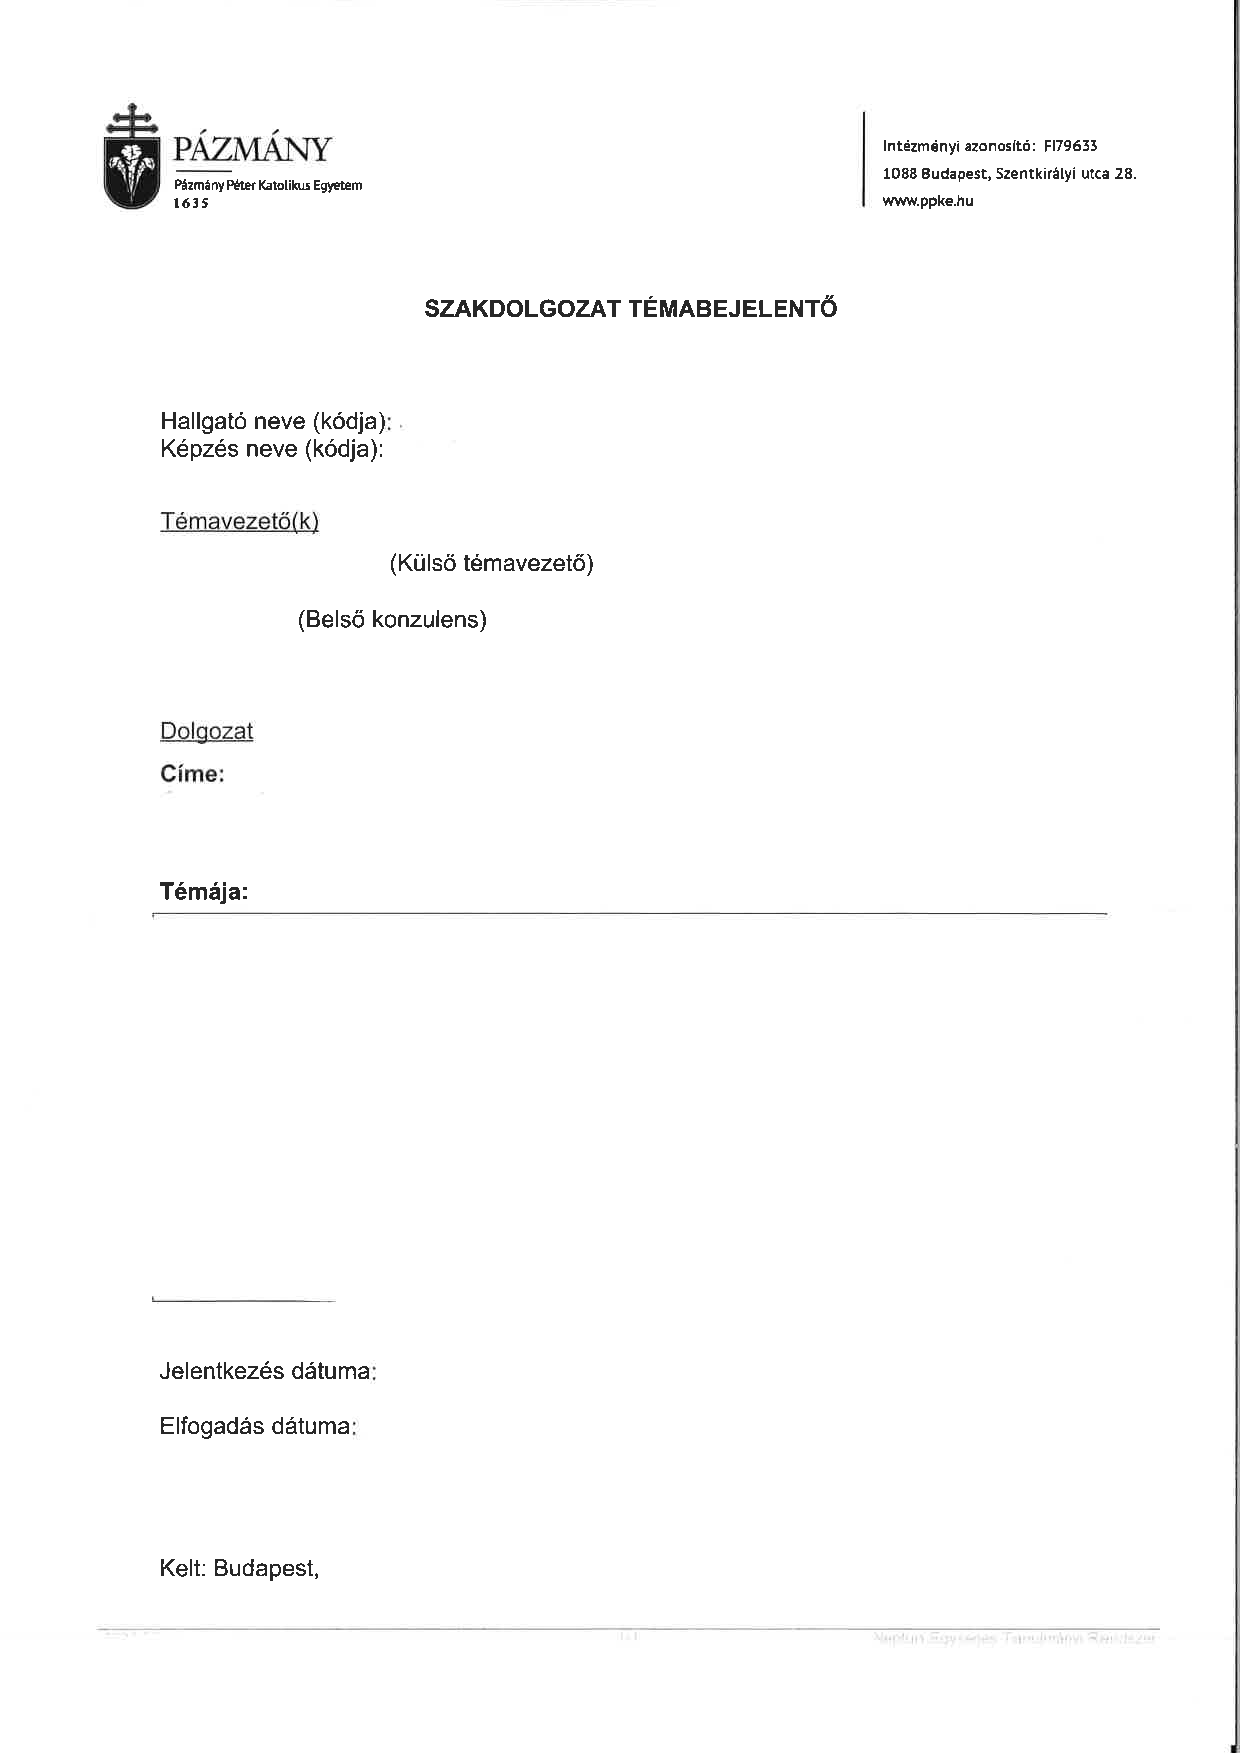
\includepdf[pages=-]{mandatory_parts/temabejelento.pdf}

% A kétoldalas témabejelentő miatt a nyilatkozat oldalszáma 3
\setcounter{page}{3}

\addcontentsline{toc}{chapter}{Nyilatkozat} 
% Itt nincs semmi teendőd

\chapter*{Nyilatkozat}
Alulírott \nev, a Pázmány Péter Katolikus Egyetem Információs Technológiai és Bionikai Karának hallgatója kijelentem, hogy ezt a szakdolgozatot meg nem engedett segítség nélkül, saját magam készítettem, és a szakdolgozatban/ csak a megadott forrásokat használtam fel. Minden olyan részt, melyet szó szerint, vagy azonos értelemben, de átfogalmazva / a dolgozat nyelvétől eltérő nyelvből fordítva, más forrásból átvettem, egyértelműen a forrás megadásával megjelöltem. Ezt a szakdolgozatot más képzésen nem nyújtottam be.
A szakdolgozatban megfogalmazott állításokért, hivatkozások helyességéért, a következtetésekért a szakmai és etikai felelősséget vállalom.

% Aláírás sor
\begin{flushright}
	\vspace*{.5cm}\par\noindent\makebox[2.5in]{\hrulefill}
	\par\noindent\makebox[2.5in][c]{\nev}
\end{flushright}

\clearpage
\addcontentsline{toc}{chapter}{Kivonat}
\chapter*{Kivonat}
% Minimum 2000 karakter, maximum két oldalas tartalmi összefoglaló a dolgozat nyelve szerinti nyelven
\paragraph{}
\lipsum[1-2] % 2 random bekezdés - ennek a helyére írd a kivonatot
\clearpage
%% Vedd ki a százalék-jelet a következő két sor elől, ha szeretnél köszönetnyilvánítást beleírni a szakdogádba/diplomamunkádba.
%\addcontentsline{toc}{chapter}{Köszönetnyilvánítás}
%\chapter*{Köszönetnyilvánítás}
% Ez egy opcionális rész

\paragraph{}
\lipsum[2] % 2 random bekezdés - ennek a helyére írd a köszönetnyilvánítást
\clearpage

% Tartalomjegyzék legenerálása
\tableofcontents
\clearpage

% Az innentől következő részek arab számozással kerülnek feltüntetésre a tartalomjegyzékben
\pagenumbering{arabic}

% Tartalmi részek - módosítsd nyugodtan
\chapter{Bevezetés}
% Csak példaként, hogy hogy működik a dolog:
\section{Szakmai háttér}
\paragraph{} Az elvégzett munka kontextusa, szakmai indoklása, motivációk, célkitűzés és az elvégzett feladatok összefoglalása.
\lipsum[5-6] % 2 random bekezdés - töröld ki

% -------------------------------------------------------------
\section{A szakdolgozat felépítése}
A szakdolgozat/diplomamunka felépítésének rövid összefoglalása:

\paragraph{2. Fejezet} Valamiről szól és most itt részletezem egy-két mondatban, hogy miről is van szó ebben a fejezetben. És most írok még egy mondatot.

\paragraph{3. Fejezet} Valamiről szól és most itt részletezem egy-két mondatban, hogy miről is van szó ebben a fejezetben. És most írok még egy mondatot.

\paragraph{4. Fejezet} Valamiről szól és most itt részletezem egy-két mondatban, hogy miről is van szó ebben a fejezetben. És most írok még egy mondatot.

\paragraph{5. Fejezet} Valamiről szól és most itt részletezem egy-két mondatban, hogy miről is van szó ebben a fejezetben. És most írok még egy mondatot.

\clearpage % Ez azért kell, hogy nehogy képek átcsússzanak a következő fejezethez
\chapter{Előzmények}
\paragraph{} irodalomkutatás, hasonló alkotások bemutatása, az ezekből a dolgozat készítője által levonható következtetések. A szakirodalom önálló, kritikai elemzése.


\section{Kapcsolódó publikációk}
\subsection{DietAI24 (Yan et al. 2025)}
\paragraph{}Ennek a tanulmánynak \cite{yan2025dietai24} az volt a célja, hogy az AI-alapú tápértékfelismerés során
megvizsgálják, hogyan hat a becsült értékek pontosságára, ha egy ellenőrzött adatbázissal támogatják a folyamat során a nagy nyelvi modellt. Az ehhez használt FNDDS adatbázis ételleírásokat és hozzájuk tartozó tápértékeket tartalmaz. A becslési folyamatot úgy tervezték meg, hogy a GPT Vision modellel először leírást készíttettek az ételről beérkező képről, majd a langchain ágens keretrendszert használva lekérdezéseket intéztek az előfeldolgozott FNDDS adatbázis felé.
Az előfeldolgozás egy vektoradatbázisba történő indexelést jelent, hogy a hasonló rekordok könnyen elérhetőek legyenek.
Az adatbázisból történő lekérdezés által kaptak egy 65 komponensű tápértékleíró vektort, ami 100g tömegre vonatkozik az adott típusú étellel kapcsolatban.
A végső lépésben azt vizsgálja a nagy nyelvi modell, hogy a megtalált lehetséges ételtípusok közül
melyek vannak valóban jelen a képen, minden egyes típushoz kiválasztja az FNDDS szabványos adagleírói közül a megfelelő adagméretet, majd a találatok és
a mennyiségek kombinációját felhasználva előállít egy a képre vonatkozó 65 elemű tápértékvektort.
Ezzel a módszerrel az ASA24 és Nutrition5k adathalmazon végzett kiértékelés során, valós vegyes ételeken, az ételtömeg és négy kulcstápanyag becslésében 63\%-os Mean Absolute Error csökkenést mértek a korábbi megoldásokhoz képest. 

Az ASA24 adathalmazon az energiabecslés átlagos abszolút hibája ételenként 47,7 kcal volt. Korlátként megemlítendő, hogy csak OpenAI GPT-modelleket vizsgáltak, és hogy az ASA24 képeinek címkéi ugyanabból az FNDDS adatbázisból származnak, amelyből a módszer is dolgozik, ami ezen az adathalmazon előnyös helyzetbe hozza. A későbbi Open-KNEAD vizsgálatban a módszer újraimplementálva, modern modellekkel, energiabecslésben mindhárom vizsgált adathalmazon a leggyengébbnek bizonyult, a Gemma-MoE modellel mérve.

\subsection{Comprehensive Evaluation of LMMs with Contextual Metadata}
\paragraph{}Ez a tanulmány \cite{coburn2025acetada} azzal foglalkozik, hogy a tápértékbecslési feladat során hogyan tudja az eredményt pontosítani, ha a kép mellett további metaadatokat is megkap a nagy nyelvi modell.
Ennek vizsgálatához az ACETADA adathalmazt (lásd~\ref{subsec:ACETADA}.~alfejezet) használták, amely GPS koordinátákat, dietetikus által ellenőrzött szöveges felsorolást az ételekről és időbélyeget tartalmaz az ételekről készült képekhez kapcsolódóan. A GPS koordinátákból szöveges kategórialeírást állítottak elő, ami jellemzi az adott helyszínt.
Emellett igyekeztek bővíteni a témában vizsgált nagy nyelvi modellek változatainak számát, ezért a négy zárt súlyú (closed-weight) modell (GPT4o, GPT-4.1, Claude 3.7 Sonnet, Gemini 2.5 Pro) mellett további négy, nyílt súlyú (open weight) modell teljesítményét is megvizsgálták (DeepSeek Janus-Pro-VL, Google Gemma-3-IT, Meta Llama-3.2-VI, Qwen 2.5-VL).
A szerzők munkájuk során arra a következtetésre jutottak, hogy a Mean Absolute Error a felhasznált kiegészítő metaadatokkal csökkenthető a vizsgált nagy nyelvi modellek használatával az ACETADA adathalmazon. 
A kontextuális metaadatok használatával, mint kiegészítő bemeneti adat, különböző érvelési promptmódszerekkel kombinálva, modellekre átlagolva a kalóriabecslés Mean Absolute Percentage Error (MAPE) értékében 4,26--10,38 százalékpontos csökkenést értek el.
További vizsgálandó területként több típusú metaadat gyűjtését említik, valamint a modellek belső adatreprezentációinak ezekhez való igazítását. 
Korlátként megemlítendő, hogy az ételfelsorolás nem a képtől független kontextus, hanem a dietetikusok által készített referenciaannotáció része, amelyből a becslések kiértékeléséhez használt tömeg- és tápértékadatok is származnak. Ennek megadásával a modell az ételek felismerését lényegében készen kapja, egy valós alkalmazásban pedig ez az információ csak a felhasználótól származhatna. Emellett modellenként a legjobb metaadat-kombinációt ugyanazon az adathalmazon választották ki, amelyen a javulást mérték, külön tesztrész nélkül, ezért a közölt javulás felső becslésnek tekinthető.



\subsection{DietDelta}
\paragraph{}Ez a tanulmány ~\cite{vinod2026dietdelta} azzal foglalkozik, hogy hogyan támogatható a képalapú tápértékbecslési feladat, ha a modell nem csak egyetlen, elfogyasztás előtti, hanem emellett egy elfogyasztás utáni képet is kap bemenetként az adott ételről. A módszerükkel kiváltani igyekeznek a mélységadatok gyűjtését. Módszerük nem nagy nyelvi modell, hanem egy CLIP (ViT-L/14) alapú képi és szöveges kódolóra épülő, keresztfigyelést és regressziós fejet használó tanított modell, amely a valós ételnevekből képzett szöveges prompt alapján ételtételenként tömeget becsül, az elfogyasztott mennyiséget pedig az elfogyasztás előtti és utáni RGB kép közötti tömegkülönbségként adja meg.
Ehhez az ACETADA, az FPB és a Nutrition5k adathalmazokat használták. Az abszolút tömegbecslésben a három adathalmazon átlagosan 14.42\%-os, az átlagos valós tömegre normalizált Mean Absolute Errort (PMAE) értek el, az elfogyasztott tömeg becslésében az ACETADA adathalmazon 14.17\%-ot.
Korlátként megemlítendő, hogy a modell a valós ételneveket kapja meg bemenetként, az ACETADA ugyanazon adathalmazának felosztásán tanították és tesztelték, valamint csak tömeget becsül, energiát nem.


\subsection{NutriMLLM (Yan et al., 2026)}
\paragraph{}Ez a tanulmány ~\cite{yan2026nutrimllm} arra keres megoldást, hogy a kereskedelmi nagy nyelvi modelleknél pontosabban oldja meg a tápértékbecslési feladatot, olyan modellekkel, amelyek szabadon elérhetőek. A szerzők szerint a kereskedelmi modellek nem alkalmasak erre a feladatra, és mérésekkel igyekeztek alátámasztani, hogy ezek olyan eredményeket adnak, amelyek helyessége statisztikailag valószínűtlen. A saját megoldásuk kidolgozásában korlátozta őket a kellő méretű tanító adathalmaz szakértők általi előállításának költsége, illetve a szükséges adathalmaz nagysága. Ezért a szintetikus adathalmaz előállítása mellett döntöttek. 1.1 millió képből álló adathalmazt hoztak létre, amelyben 65 tápérték paraméter ír le minden egyes ételről generált képet, amelyeket az NHANES 24 órás étkezési naplóinak szöveges ételleírásaiból generáltak, a tápértékcímkéket pedig az FNDDS adatbázisból vették.

Ezután ennek segítségével finomhangolták a Qwen3-VL és GLM-4.6V-Flash szabadon elérhető nagy nyelvi modelleket, ezzel létrehozva a NutriMLLM modellt. 
Ennek a legnagyobb változata elérte, illetve esetenként meghaladta a kereskedelmi modellek (GPT-5, Gemini 3, and Claude Sonnet 4.5) teljesítményét a feladatban.
A szöveges ételleírásokat tartalmazó NutriBench adathalmazon végzett kiértékelés során a NutriMLLM legnagyobb (Qwen3-VL-30B alapú) változatának használhatatlan becslések aránya 0-0.4\% tartományra csökkent, amíg a kereskedelmi modellek 0.1-0.8\%-os tartományban mozogtak. A nem finomhangolt szabadon elérhető modellek esetében a használhatatlan becslések aránya magasabb, 5.9-39.2\% tartományban mozgott.
A numerikus pontosságot a szerzők az elutasításra korrigált szimmetrikus átlagos abszolút százalékos hibával mérték (SMAPE).
Ez 0\% és 200\% között mozog, és a hiányzó becsléseket büntetve megakadályozza, hogy a modell a nehéz esetekre való válaszmegtagadással javítson az eredményén.
A finomhangolás hatására az ASA24 adathalmazon a Qwen3-VL-30B 65 tápanyagra átlagolt SMAPE értéke 133.3\%-ról 109.8\%-ra csökkent. Ez alacsonyabb, mint a kereskedelmi modellek SMAPE értékei: Claude Sonnet 4.5: 118.0\%; Gemini 3: 125.5\%; GPT-5: 137.9\%. A SNAPMe adathalmazon a Qwen3-VL-30B finomhangolt modell SMAPE értéke 108.5\%-ról 91.2\%-ra csökkent, szintén a kereskedelmi modelleknél alacsonyabb értéket elérve. A kereskedelmi modellek SMAPE értékei a fentebb megadott sorrendet követve a SNAPMe adathalmazon: 94.7\%, 95.7\%, és 102.6\%.
Korlátként megemlítendő, hogy a 65 tápanyagra átlagolt SMAPE-t főként a mikrotápanyagok határozzák meg, így az energiabecslés pontosságáról keveset mond. A NutriBench energiabecslésében a kereskedelmi modellek pontosabbak voltak (például Gemini 3: 25,3\%, NutriMLLM-30B: 47,4\% SMAPE). A tanulmányt a DietAI24 szerzőcsoportja készítette.



\subsection{Open-KNEAD (Coburn et al., 2026)}
\paragraph{}Ez a tanulmány ~\cite{coburn2026openknead} azt a kérdést veti fel a nagy nyelvi modellekkel végzett tápértékbecslési feladat során, hogy egy tápértéksűrűség-adatbázis vajon minden esetben hozzájárul-e a feladat megoldásának pontosságához. Ennek vizsgálatára olyan folyamatot terveztek és futtattak, amely egyaránt végez közvetlen, prompt-alapú és ún. RAG módszeres becslést egy tetszőleges, szabadon elérhető nagy nyelvi modell segítségével.
Azt, hogy az energiabecslést RAG módszerrel vagy közvetlenül a bemeneti képből becslik, előre rögzítették aszerint, hogy a tápértékadatbázis mennyire fedi le az adott adathalmaz konyháját. Az adagbecslés minden esetben az adatbázisra támaszkodó ágból származik.
Méréseik alapján összehasonlítható a közvetlen és az ún. RAG alapú becslés hat különböző kombinációja a fenti megközelítéssel a Nutrition5k, az OmniFood8K és az ACETADA adathalmazokon, Gemma-E4B, Qwen-9B, Gemma-MoE, Gemma-31B, Qwen-35B modellekkel. 
Az energiabecslést csak az ACETADA esetén vették a közvetlen becslésből.
Megállapították, hogy a mai nagy nyelvi modellek közvetlen becslése energiában eléri vagy meghaladja a teljes RAG-alapú folyamatét. Az adatbázis haszna az adagbecslésben és a tételesen ellenőrizhető eredményben jelentkezik.
A legnagyobb pontosságjavulást az ACETADA adathalmazon tudták elérni a módszerükkel: a helyben futó Gemma-31B 147g teljes étkezésadagondként számított Mean Absolute Errort ért el, ami ~30\%-kal jobb a gpt-5.5 direkt becslésénél (212 g).
A tanulmány az ACETADA és a DietDelta szerzőivel közös kutatócsoportból származik.


\subsection{Vision-Language Models for Image-Based Dietary Assessment: A Benchmark of Accuracy, Cost, and Prompt Strategies Across Ten Models}
\paragraph{}Ez a tanulmány ~\cite{sterling2026vlm} prompt stratégiák és nagy nyelvi modellek kombinációjának hatékonyságát mérte: öt promptolási megközelítést a Gemini 2.0 Flash modellel vizsgáltak, majd a legjobbat kilenc különböző nagy nyelvi modellen alkalmazták. Emellett egy kereskedelmi API-t is használtak egy esetben a nagy nyelvi modellek helyett. A mérés során a Nutrition5k adathalmaz RGB adatokat tartalmazó, felülnézeti képeit használták. 

Ezen képek közül metaadat-alapú kritériumokat figyelembe véve  3229-at választottak ki (31 elavult összetevő, 2 üres tányér, 228 nulla vagy hiányzó tömeg).

A kereskedelmi modellek közül nyolc félét vizsgáltak: Gemini 2.0 Flash, 2.5 Flash, 3.0 Flash és 3.1 Flash Lite; GPT-4o, GPT-4o-mini és GPT-5 Mini; Claude Haiku 4.5. A szabadon elérhetőek közül kizárólag a Qwen2-VL-7B-t.
A mérések során használt ételfelismerésre készült kereskedelmi szolgáltatás a FatSecret API volt. A modellek a felismert összetevőket, azok becsült tömegét és kalóriatartalmát adták válaszul a bemeneti képre.
A promptolási stratégiák a következőek voltak:
P1 - Csak a feladatot és a kimeneti formátumot adja meg;
P2 - Először a tömeg becslése, ebből a tápérték;
P3 - Nem használ sztenderd adagtömeg-értékeket az adatbázisból, hanem a képen látható adagot közvetlenül a becsli, ebből tápértéket számol;
P4 - Korlátokat adtak meg, amiken belül a becslés elfogadható, reális;
P5 - Első lépésben P3, majd egy önellenőrzés a modell által.

A legjobb eredményeket a P3 prompttal érték el. A teljes összehasonlításban a Gemini 3.0 Flash érte el a legjobb kalóriabecslést (CCC 0,767, MAE 80,7 kcal).
Korlátként megemlítendő, hogy a promptokat csak egy modellen vizsgálták, és a nem feldolgozható válaszokat kizárták a kiértékelésből (a GPT-5 Mini 213 képre nem adott értelmezhető választ).

\section{Kapcsolódó adathalmazok}

\subsection{ASA24}
\paragraph{}Az ASA24 \cite{subar2012asa24} az amerikai National Cancer Institute által fejlesztett, webalapú 24 órás étkezési napló vezetését támogató szoftver. Kitöltéskor a felhasználó az elfogyasztott mennyiséget referenciaképek közül választva adja meg. A tanulmányban használt adathalmaz ezeket a porcióméret-képeket és a hozzájuk tartozó FNDDS kódokat tartalmazza. A képeket az eszköz fejlesztői egységes, kontrollált körülmények között készítették, és mindegyik egy FNDDS-ételkódhoz és egy meghatározott porcióhoz tartozik, így minden képhez pontos tápanyagérték rendelhető. Ugyanazt az ételt jellemzően több, fokozatosan növekvő adagban is ábrázolják, ezért a porcióbecslés külön is vizsgálható. Fontos korlát, hogy a képek nem valós étkezési helyzetben készültek, hanem jellemzően egyetlen ételt mutatnak ideális fotózási körülmények között.

\subsection{NutriBench}
\paragraph{}A NutriBench \cite{dhaliwal2025nutribench} szöveges adathalmaz, amely képek helyett étkezések természetes nyelvű leírásait tartalmazza. A 11857 leírás valós étkezési felmérésekből készült, az amerikai What We Eat in America felmérésből, valamint a FAO/WHO GIFT adatbázisból, összesen 11 ország adataival. A leírásokat GPT-4o-mini fogalmazta meg a felmérésekben rögzített ételekből és mennyiségekből, a szerzők pedig ellenőrizték, hogy minden étel és adag szerepeljen bennük. A mennyiségek egy része grammban, más része hétköznapi mértékegységben (például „fél csésze") van megadva. Minden leíráshoz szénhidrát-, fehérje-, zsír- és energiaérték tartozik, az amerikai részben az FNDDS adatbázis 2017--2018-as kiadása alapján.

\subsection{DFood-TJ}
\paragraph{}A DFood-TJ adathalmaz~\cite{jin2026dfoodtj} négy részből áll: 3932 képet tartalmaz 187 ételtípusról kézi poligonannotációval, 284 933 képet 351 kategóriába rendezve, ételfelismerési, kategorizálási feladatokhoz, 351 ételtípus sűrűség- és tápanyagsűrűség-értékeit adja meg, valamint szénhidrát-, zsír-, fehérje-, rost- és energiatartalmat ad meg 3280 képhez, amelyek 91 kórházban kezelt beteg étkezéseiről, 101 ételtípusról készültek; ezek tápértékét a mért ételtömegekből számították. Az adathalmaz kifejezetten a cukorbetegség kezelését támogató táplálkozáselemzés céljából készült. A szerzők indoklása szerint a legtöbb adathalmazzal foglalkozó publikáció a témában felismerési vagy szegmentálási feladatokra készült, és a kínai konyhára vonatkozó, tápanyagbecslésre alkalmas adat különösen ritka. Ennek a hiányát igyekeztek pótolni.

\subsection{ACETADA}
\label{subsec:ACETADA}
\paragraph{}Az ACETADA adathalmaz \cite{coburn2025acetada} egy ausztráliai, kontrollált étkeztetéses vizsgálatból származik, amelyben 152 felnőtt résztvevő három, egymástól egy hétre eső napon napon át laboratóriumban elkészített reggelit, ebédet és vacsorát fogyasztott, az elfogyasztott mennyiséget pedig a kutatók 0,1g pontossággal megmérték. A résztvevők az étkezések előtt és után telefonnal fényképezték le az ételt. A képeken méretarány-jelölő is szerepel, és mindegyikhez időbélyeg, valamint, ha elérhető volt, GPS-koordináta tartozik. A képeket dietetikusok ellenőrizték: azonosították a látható ételeket, és az ausztrál AUSNUT 2011--2013 adatbázis alapján meghatározták azok tömegét, energia- és makrotápanyag-tartalmát. A címkék az elfogyasztott mennyiséget írják le, ezért az étkezés előtti képen látható adag ennél nagyobb is lehet. Az Open-KNEAD szerzői~\cite{coburn2026openknead} ugyanezt az adathalmazt dietetikus által ellenőrzött tálalt mennyiségként írják le, ami ellentmond a forráscikknek.

\subsection{Nutrition5k}
\paragraph{}A Nutrition5k \cite{thames_nutrition5k_2021} adathalmaz nagyjából húsz ezer rövid videót tartalmaz megközelítőleg öt ezer különböző ételről. Az ételek több mint 250-féle hozzávalóból készültek. Mindegyikhez tartozik lista a hozzávalóikról és azok mennyiségéről. Emellett tartalmazza minden étel makronutriens-információit a USDA Food and Nutrient Database \cite{usda_fndds_2010} formátumának megfelelően. 3500 ételhez az adathalmazban tartozik úgynevezett RGB-D kép, amely mélységadatot biztosít, ezeket egy Intel RealSense kamerával rögzítették. Az adathalmazt a készítők tanító és teszt részre osztották, 90\%-10\% arányban.
Az ételek tömegének szórása 161g, energiatartalmuk szórása 220 kcal, átlagosan 5.7 eltérő hozzávalót tartalmaznak, a legtöbbet tartalmazó 35-féléből készült.
Sterling et al.~\cite{sterling2026vlm} humán validációja szerint az összetevőlisták az összetettebb ételeknél gyakran hiányosak, ezért az összetevő-felismerés ezekhez mért pontossága alulbecsli a modellek valós teljesítményét.

\subsection{OmniFood8k}
\paragraph{}Az OmniFood8K \cite{yu2026omnifood8k} 8036 kínai ételt tartalmazó, multimodális adathalmaz, amely a nyugati ételekre épülő adathalmazok hiányosságát hivatott pótolni. Az ételek elkészítése előtt a szerzők minden hozzávalót lemértek és lefényképeztek, a főzést videóra vették, a receptet szövegesen rögzítették, a kész ételt pedig hat kamerával, egyszerre több nézőpontból fényképezték le. A tápértékadatok (energia, tömeg, fehérje, zsír és szénhidrát) a hozzávalók mért tömegéből, tápanyag-adatbázis alapján számított értékek. A felvételek egységes, rögzített kameraállásokból készültek.

\subsection{SNAPMe}
\paragraph{}A SNAPMe \cite{larke2023snapme} hétköznapi körülmények között készült étkezési fotókat tartalmaz. A vizsgálat 95 résztvevője legfeljebb három napon át minden elfogyasztott ételt lefényképezett mobiltelefonos alkalmazással, és ezzel párhuzamosan az ASA24 2020-as változatában étkezési naplót vezetett. A nem csomagolt ételekről evés előtt és után is készült fotó, az egyadagos csomagolt termékekről pedig a csomagolás elejéről és az összetevőlistáról. Az adatbázis 3311 fotót és 275 étkezési naplót tartalmaz. A referenciaértékek így nem mérlegelésből, hanem a résztvevők önbevallásából származnak.

\subsection{FNDDS}
\paragraph{}Az FNDDS (Food and Nutrient Database for Dietary Studies) \cite{usda_fndds_2010} az amerikai mezőgazdasági minisztérium (USDA) által fenntartott tápanyag-adatbázis, amely a What We Eat in America / NHANES felmérésekben rögzített ételek tápértékét adja meg. Minden ételhez nyolcjegyű ételkód, szöveges leírás, szabványos adagméretek és 65 tápanyag- és ételkomponens-érték tartozik 100 grammra vonatkoztatva. A 2019--2020-as kiadás 5624 ételt tartalmaz. A bemutatott tanulmányok közül a DietAI24, a NutriMLLM és az Open-KNEAD erre épül, és az ASA24, a SNAPMe, valamint a NutriBench amerikai részének címkéi is ebből származnak. Mivel az adatbázis az amerikai étrendet fedi le, más konyhák ételeinél szisztematikus eltéréssel kell számolni.

\clearpage % Ez azért kell, hogy nehogy képek átcsússzanak a következő fejezethez

\chapter{Tervezés}
Alkamazmazott módszertan/technológiák ismertetése: A dolgozat témájához illeszkedve kell részletezni a feladat megoldásához, megvalósításához kapcsolódó szakmai hátteret.

\section{Döntési lehetőségek értékelése}
\paragraph{}
\lipsum[9] % 1 random bekezdés - töröld ki

\section{Választott megoldások indoklása}
\subsection{Megoldás1}
\paragraph{}
\lipsum[10] % 1 random bekezdés - töröld ki
\paragraph{}
\lipsum[11] % 1 random bekezdés - töröld ki

\subsection{Megoldás2}
\paragraph{}
\lipsum[12] % 1 random bekezdés - töröld ki
\paragraph{}
\lipsum[13] % 1 random bekezdés - töröld ki

\clearpage % Ez azért kell, hogy nehogy képek átcsússzanak a következő fejezethez
\chapter{Eredmények}
A megtervezett műszaki alkotások értékelése, kritikai elemzése, továbbfejlesztési lehetőségek. 

\section{Képek}
\paragraph{}Itt szerepeljen most pár kép példaként, hogy hogyan lehet őket beszúrni. Fontos, hogy a \LaTeX\ leegyszerűsíti a dolgodat azzal, hogy kitalálja, hogy hova fér el a kép, cserébe nincs abba kifejezetten sok beleszólásod, hogy pontosan hova kerüljön a kép. Ha fontos neked, hogy megmondd, hogy pontosan hol legyen a kép, akkor Google a barátod... Az is fontos, hogy a szövegben minden képre és táblázatra hivatkozz. Például a ~\ref{fig:cat}. ábra egy cicás képet mutat. A szövegben leírtak láthatóak \az ~\ref{fig:rat}. ábrán, illetve \az~\ref{fig:dog1}. és \ref{fig:dog2}.~ábrákon.


\begin{figure}
  \centering
  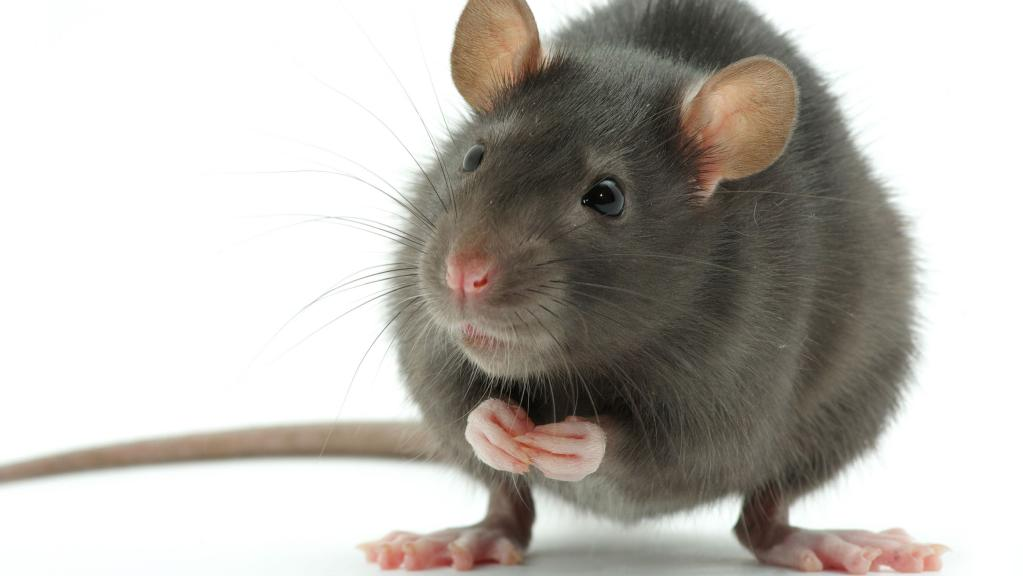
\includegraphics[width=0.6\textwidth]{rat}
  \caption{Random kép egy patkányról. A kép szélessége a lap szélességének 0.6-szorosa. Kép forrása: http://www.mmbcc.org.au~\cite{noauthor_ratification}.}
  \label{fig:rat}
\end{figure}

\begin{figure}
  \centering
  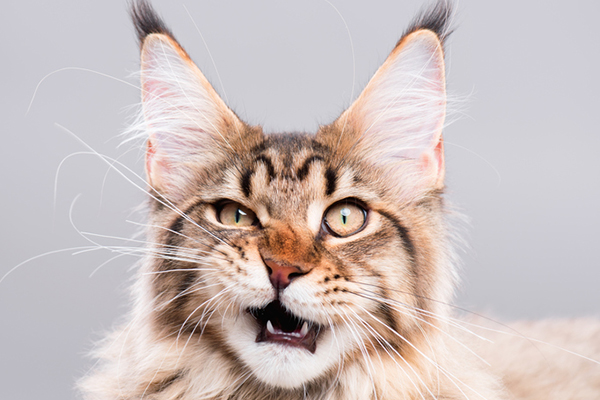
\includegraphics[width=\textwidth]{cat}
  \caption{Random kép egy macskáról. A kép szélessége megegyezik a lap szélességével. Kép forrása: www.theodysseyonline.com~\cite{noauthor_20_2017}.}
  \label{fig:cat}
\end{figure}

\begin{figure}
    \begin{minipage}[c]{0.45\linewidth}
        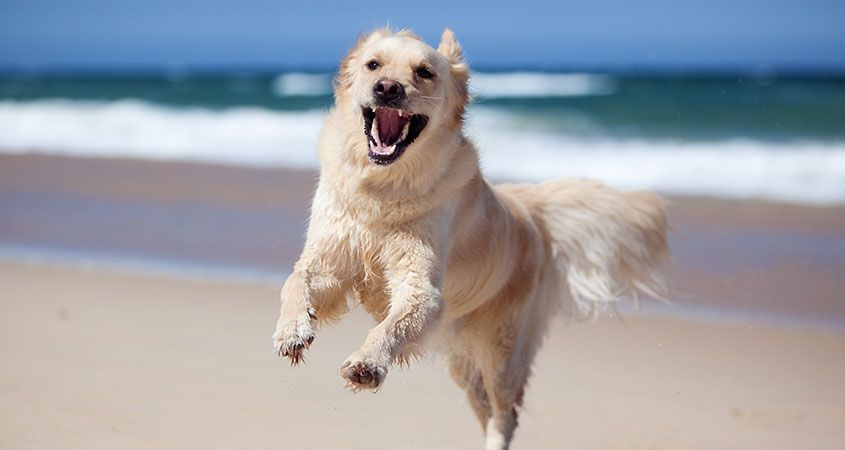
\includegraphics[width=\linewidth]{dog1}
        \caption{Random kép egy kutyáról egy másik kutyás kép bal oldalán. Kép forrása: www.huffingtonpost.ca~\cite{noauthor_get_2016}.}
        \label{fig:dog1}
    \end{minipage}
    \hfill
    \begin{minipage}[c]{0.45\linewidth}
        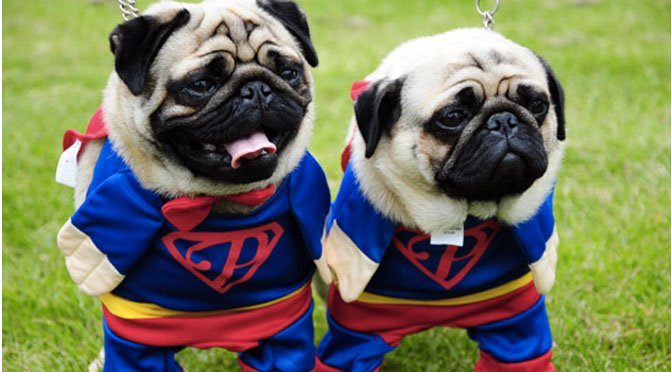
\includegraphics[width=\linewidth]{dog2}
        \caption{Random kép egy kutyáról egy másik kutyás kép jobb oldalán. Kép forrása: imgur.com~\cite{imgur_superman_nodate}.}
        \label{fig:dog2}
    \end{minipage}
\end{figure}

\section{Táblázat}
\paragraph{}Legyen akkor már példa táblázat beillesztésére is. Az \ref{tab:features}.~táblázat a saját szakdogám egy random részéről került beillesztésre.


\begin{table}
\centering
\begin{tabular}{|l|l|l|}
\hline
\rowcolor[HTML]{C0C0C0} 
Positive for... & Negative for... & Number of features \\ \hline
AF & other & 37 \\ \hline
other & normal & 25 \\ \hline
other & AF & 11 \\ \hline
normal & AF & 11 \\ \hline
AF & normal & 1 \\ \hline
\end{tabular}
\caption{Random táblázat.}
\label{tab:features}
\end{table}

\clearpage % új oldalt kezd. A \newline hasonló parancs, de a \clearpage gondoskodik arról, hogy a fentebb beszúrt képek és táblázatok, az alábbi kódok előtt szerepeljenek mindenképp.

\section{Hivatkozás}
Legyen most itt egy hivatkozás Thompson cikkére~\cite{thompson_kennedy_1996}, aminek az adatai a hivatkozasok.bib fájlban található. A hivatkozasok.bib fájlt egyébként érdemes a következő oldal segítségével legenerálni: \url{http://www.citethisforme.com/ieee}. A "More" menü alatt található az "Export" almenüben az "Export as BibTeX" parancs, amivel le lehet tölteni a megfelelő formátumban. Másik opció a zotero használata, ami talán még egyszerűbb, cserébe telepíteni kell: \url{https://www.zotero.org/support/getting_stuff_into_your_library}.

\section{Szövegformázás}
\paragraph{}
\textbf{Legyen itt egy mondat vastagon szedetten.
Meg egy másik, ami \underline{aláhúzásra} is példa + \textit{dőlt betű példa is}.} Utána pedig egy hosszabb térköz.

\vspace{1.5cm}

\section{Forráskód}
Legyen itt egy kis forráskód is:
\lstset{language=Pascal,caption={A Pascal kódrészlet képaláírása.}}
\begin{lstlisting}
for i:=maxint to 0 do
begin
{ do nothing }
end;
Write('Case insensitive ');
Write('Pascal keywords.');
\end{lstlisting}

Meg egy másik, ami teljes fájlt mutat meg, és kódszínezést is mutat:
\lstset{
    language=Python,
    caption={A Python kódrészlet képaláírása.},
    keywordstyle=\color{red},
    stringstyle=\color{blue},
    commentstyle=\color{green},
    morecomment=[l][\color{magenta}]{\#}
}
\lstinputlisting{contents/z_example.py}

\section{Felsorolás}
Végül mutatok egy felsorolást is:
\begin{enumerate}
    \item Első elem
    \begin{itemize}
        \item Valami
        \item Megint valami
        \item Meg valami más
    \end{itemize}
    \item Második elem
    \begin{itemize}
        \item asdf
        \item qwertz
        \item yxcv
    \end{itemize}
    \item Harmadik elem
    \begin{itemize}
        \item Itt a vége
    \end{itemize}
\end{enumerate}

\section{Egyenletek}
És akkor már csak az egyenletek vannak hátra. Itt van egy olyan egyenlet, ami nem kezd új sort: $a^2 + b^2 = c^2$ vagy $\sum_{i = 0}^{n}a_i - \int_{0}^{\pi}f(x)dx$. De van olyan is, ami új sort kezd (két dollár-jellel kezdem és fejezem be): $$\frac{-b\pm\sqrt{b^2-4ac}}{2a}.$$
Ha pedig arra van szükségem, hogy számozott legyen az egyenlet, és pl hivatkozni tudjak a \ref{eq:bonyolult}.~egyenletre, akkor így lehet csinálni:
\begin{equation} \label{eq:bonyolult}
    \sum_{i=1}^{\left[\frac{n}{2}\right]}\binom{x_{i,i+1}^{i^{2}}}
    {\left[\frac{i+3}{3}\right]}\frac{\sqrt{\mu(i)^{\frac{3}{2}}(i^{2}-1)}}{\sqrt[3]{\rho(i)-2}+\sqrt[3]{\rho(i)-1}}
\end{equation}

Egyenletek \LaTeX kódjának írását hamar elsajátíthatja az ember némi googlizás árán, viszont van erre online szerkesztő is: \url{http://www.hostmath.com/}.

\newpage

\section{Hosszú idézet}
\paragraph{Random szöveg az idézet előtt.}\lipsum[2]
\begin{displayquote}
    The 2017 PhysioNet/CinC Challenge aims to encourage the development of algorithms to classify, from a single short ECG lead recording (between 30 s and 60 s in length), whether the recording shows normal sinus rhythm, atrial fibrillation (AF), an alternative rhythm, or is too noisy to be classified.
    
    Previous studies concerning AF classification are generally limited in applicability because 1) only classification of normal and AF rhythms were performed, 2) good performance was only shown on carefully-selected often clean data, 3) a separate out of sample test dataset was not used, or 4) only a small number of patients were used. 
    It is challenging to reliably detect AF from a single short lead of ECG, and the broad taxonomy of rhythms makes this particularly difficult. 
    In particular, many non-AF rhythms exhibit irregular RR intervals that may be similar to AF. 
    In this Challenge, we treat all non-AF abnormal rhythms as a single class and require the Challenge entrant to classify the rhythms as 1) Normal sinus rhythm, 2) AF, 3) Other rhythm, or 4) Too noisy to classify.
\end{displayquote}
\begin{flushright}-------------- Introduction to \textit{Computing in Cardiology Challenge of 2017}\end{flushright}

\paragraph{Random szöveg az idézet után.}\lipsum[2]

\clearpage % Ez azért kell, hogy nehogy képek átcsússzanak a következő fejezethez
\chapter{Összefoglalás}
Az elvégzett feladatok összefoglalása, összehasonlítva a kitűzött célokkal. Továbblépési lehetőségek, kérdések megadása, kitekintés.

\section{Feladat}
A kitűzött célok felsorolása, reflexió mindre.
\section{Eredmények}
Egy bekezdésben összefoglalva az eredmények fejezet, következtetések levonása.
\section{Jövőbeli tervek}
Egy bekezdésben, a mérések és a kiértékelés után.

% Hivatkozásjegyzék/bibliográfia
\printbibliography
\addcontentsline{toc}{chapter}{Felhasznált irodalom}

% Mellékletek - ha nincs mellékleted, töröld az alábbi részt
\appendix
\chapter{Melléklet}
\textbf{Megértést segítő képek, ha szükséges, ide elvileg lehet nem csak saját munkát
a sablon szerint.}
\iffalse
Ide kerülnek azok a dolgok, amik segítik a dolgozat megértését, de  1) nem a te munkád, 2) nem feltétlenül szükséges a megértéshez, vagy 3) simán csak érdekességek. Na, meg ha rengeteg képed van ugyanarról a dologról, és nem szeretnéd ezzel teletömni a szakdogád, akkor ide is nyugodtan berakhatod őket.
\fi

\end{document}
